\documentclass[11pt,answers]{exam}

% Load useful packages
% Read in necessary packages
\usepackage{import}
\usepackage{amsmath}
\usepackage{amsfonts}
\usepackage{amssymb}
\usepackage{graphicx}
\usepackage{hyperref}
\usepackage{color}
\usepackage{subfigure}
\usepackage{tikz}

% Set various options for exam package
\shadedsolutions % defines the style of the solution environment

% Set lesson name, etc.
\newcommand{\coursename}{Math 312}
\newcommand{\lessonname}{Problem Set 2}
\newcommand{\duedate}{9 February 2016}
\newcommand{\names}{Tate Maki-Waller, Sam Gleason, Ian Gallmeister}

% Set headers/footers to look nice
\pagestyle{headandfoot}
\firstpageheader{\textbf{\large \coursename\ \lessonname}}{}{\textbf{\large Due \duedate}}
\firstpageheadrule
\runningheader{\textbf{\large \coursename\ \lessonname}}{}{\textbf{\large Due \duedate}}
\runningheadrule
\firstpagefooter{\names}{}{Page \thepage\ of \numpages}
\firstpagefootrule
\runningfooter{\names}{}{Page \thepage\ of \numpages}
\runningfootrule

% Define commands related to marking up content
\newcommand{\source}[1]{}

% Define commands related to general mathematical style
\renewcommand{\exp}[1]{e^{#1}}

\renewcommand{\theenumi}{(\alph{enumi})}
\renewcommand{\labelenumi}{\theenumi}
\renewcommand{\thequestion}{\arabic{question}}
\renewcommand{\questionlabel}{(\thequestion)}
%%%%%%%%%%%%%%%%%%%%%%%%%%%%%%%%%%%%%%%%%%%%%%%%%%%%%%%%%%%%

\begin{document}
\begin{questions}

\addtocounter{question}{8}

\question
An unstable nucleus is radioactive. At any instant, it can emit a particle, transforming itself into a different nucleus in the process. In a sample of $^{238} U$ (uranium-238), a certain percentage of the nuclei will decay during a given observation period. If at time $t$ a sample contains $N(t)$ radioactive nuclei, then we expect that the number of nuclei that decay in the time interval $\Delta t$ will be (approximately) proportional to $N$ and $\Delta t$. That is, if there are more nuclei in the sample, more will decay in a given amount of time. But also, if we wait longer, more will decay. Mathematically, we may write

\[
N(t + \Delta t) = N(t) - \lambda N(t) \Delta t
\]
where $\lambda$ is a constant of proportionality.

\begin{enumerate}
\item By taking the limit of infinitesimal $\Delta t$ and recalling the definition of a derivative, derive the differential equation that $N(t)$ satisfies.
\begin{solution}

First we need to find the difference between $N(t + \Delta t)$ and $N(t)$ in terms of $\Delta t$.  Then, sending $\Delta N$ and $\Delta t$ to 0 means we can replace them with $dN$ and $dt$ to get our differential equation.

\begin{align*}
N(t + \Delta t) - N(t) &= - \lambda N(t)\Delta t \\
\lim_{\Delta t \to 0} \Delta N &= -\lambda N(t) \Delta t \\
dN &= -\lambda N(t) dt
\end{align*}

\end{solution}

%%%%%%%%%%%%%%%%%%%%%%%%%%%%%%%%%%%%%%%%%%%%%%%%%%%%%%%%%

\item Suppose that $N(0) = N_0$. Solve the initial value value problem.
\begin{solution}

By separation of variables, we can antidifferentiate the result from part (a) and use the initial condition to find $N(t)$.

\begin{align*}
N(0) &= N_0\\
\frac{dN}{N} &= \lambda dt \\
\ln{N} &= Ce^{\lambda t} \\
N_0 = Ce^0 &\Rightarrow C = N_0 \\
N(t) &= N_0e^{\lambda t}
\end{align*}
\end{solution}

%%%%%%%%%%%%%%%%%%%%%%%%%%%%%%%%%%%%%%%%%%%%%%%%%%%%%%%%%
\pagebreak
\item The half-life $T_{1/2}$ of a substance is the amount of time it takes for half of a sample of the substance to decay. Derive a formula for $T_{1/2}$
\begin{solution}

After $T_{1/2}$ years, there will be $N_0 / 2$ amount of $^{238}U$ assuming we start from some amount $N_0$.

\begin{align*}
T_{1/2} \rightarrow N(T_{1/2}) &= N_0e^{\lambda(T_{1/2})} = \frac{N_0}{2}\\
\ln{\frac{1}{2}} &= \lambda T_{1/2} \\
T_{1/2} &= - \frac{\ln{1/2}}{\lambda}
\end{align*}

\end{solution}

%%%%%%%%%%%%%%%%%%%%%%%%%%%%%%%%%%%%%%%%%%%%%%%%%%%%%%%%%

\item The half-life of $^{238} U$ is $4.47 \times 10^7$ yr. Suppose that 1000 mg of $^{238} U$ are present initially.  Determine the time for this sample to decay to 100 mg.
\begin{solution}

First, we need a value for $\lambda$

\[
4.47 \times 10^7 = - \frac{\ln{1/2}}{\lambda} \Rightarrow \lambda = -\frac{\ln{1/2}}{4.47 \times 10^7}
\]

Now, we can plug that in for $\lambda$ and solve for $t$.  The equation below skips the first step as a decay equation can either be of the form $N_f = N_0 e^{(???)}$ or $\frac{N_f}{N_0} = e^{(???)}$

\begin{align*}
\frac{1}{10} &= e^{\frac{\ln{(1/2)}t}{4.47\times 10^7}}\\
t &= \frac{1/10}{1/2}4.47\times 10^7 \\
t &= 1.484 \times 10^8 yr
\end{align*}
\end{solution}
\end{enumerate}

\question The Felix Problem
\begin{solution}

\end{solution}

\question Hailstones
\begin{solution}

\end{solution}

\question Complex Unit Circle
\begin{solution}

\begin{tikzpicture}
\draw(0,0) -- (2,0);
\draw(3,0) -- (5,0);
\draw(6,0) -- (8,0);
\draw(1, -1) -- (1, 1);
\draw(4, -1) -- (4, 1);
\draw(7, -1) -- (7, 2);
\draw[->](1,0) -- (1,1);
\draw[->](4,0) -- (4.707, 0.707);
\draw[->](7,0) -- (7.707, 1.707);
\end{tikzpicture}

The first set of axes is for $e^{\pi/2} = \cos(\pi/2) + i\sin(\pi/2) = i$.  The second is $e^(\pi/4) = \cos(\pi/4) + i\sin(\pi/4) = \sqrt{2}/2 + i\sqrt{2}/2$.  Their sum is the third, and because the two vectors are the same length, the angle of their sum is the average of the two angles, $3\pi/8$ in this case.  That vector has the value $\sqrt{2}/2 + i(1 + \sqrt{2}/2)$.  The tangent of that angle would then be 
\[
\frac{1 + \sqrt{2}/2}{\sqrt{2}/2} = \frac{\sqrt{2}/2 + 1}{1} = \frac{\sqrt{2}}{2} + 1
\]

\end{solution}

\question Using complex numbers, derive an identity that expresses $\cos(3\theta)$ in terms of $\sin(\theta)$ and $\cos(\theta)$.
\begin{solution}

To do this problem, we need to know that $\cos{\theta} = \frac{1}{2}\left(e^{i\theta} + e^{-i\theta} \right)$ and Euler's formula.  Then the question is just a matter of algebra.  Yay algebra!

\begin{align*}
\cos(3\theta) &= \frac{1}{2}\left( e^{3i\theta} - e^{-3i\theta} \right) \\
&= \frac{1}{2}\left( \left( e^{i\theta} \right)^3 + \left( e^{-i\theta} \right)^3 \right) \\
&= \frac{1}{2}\left( \left( \cos{\theta} + i\sin{\theta} \right)^3 + \left( \cos{\theta} - i\sin{\theta} \right)^3 \right)\\
&= \frac{1}{2} \left[ \left(\cos^2\theta + 2i \cos{\theta}\sin{\theta} - \sin^2\theta \right) \left(\cos{\theta} + i\sin{\theta}\right) \right. \\
&\hbox{\hspace{1.5em}}+ \left. \left( \cos^2\theta - 2i\cos{\theta}\sin{\theta} - \sin^2\theta \right)\left( \cos{\theta} - i\sin{\theta} \right) \right] \\
&= \frac{1}{2}\left( \cos^3\theta + 3i \cos^2\theta\sin{\theta} - 3\cos{\theta}\sin{\theta} - i\sin^3\theta \right.\\
&\hbox{\hspace{2em}}+ \left. \cos^3\theta + ^-3i\cos^2\theta\sin{\theta} - 3 \cos{\theta}\sin^2\theta + i\sin^3\theta \right) \\
&= \frac{1}{2}\left( 2\cos^3\theta - 6\cos\theta\sin^2\theta \right)\\
&= \cos^3\theta - 3\cos{\theta}\sin^2\theta
\end{align*}
\end{solution}

\pagebreak
\question IVT Problem for a Complex $z$

\begin{solution}
MatLab Code:
\begin{verbatim}
function [t, z] = imaginarysolve

%Start and end times:
t0 = 0;
tf = 4;

%Initial Condition:
z0 = 1 + 1i;

%Solve
[t, z] = ode45(@dzdt, [t0, tf], z0, []);
end

function z = dzdt(t, z)
z = (-1 + 10i)*z;
end
\end{verbatim}
Images for (a) at the end.

Part (b)
\begin{align*}
z & = x + iy \\
\frac{dz}{dt} &= (-1 + 10i)z \\
&= (-1 + 10i)(x + iy)\\
&= x(-1 + 10i) - y(10 + i)
\end{align*}

\end{solution}

\pagebreak

\begin{verbatim} \begin{solution} ... \end{solution} \end{verbatim} doesn't work with figures.
%\begin{solution}
\begin{figure}[h]
    \centering
    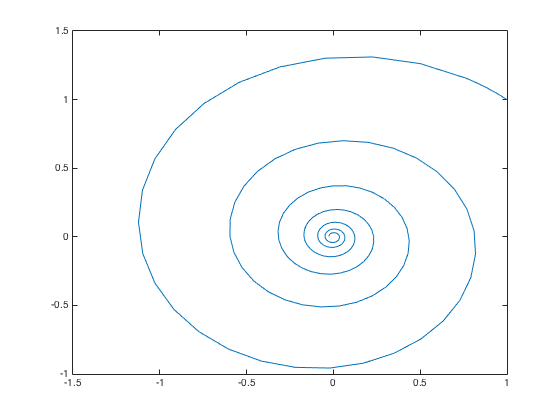
\includegraphics[width = 0.65\textwidth]{zRvszi.png}
    \caption{Graphing Z - Real and Imaginary axes}
    \label{fig:my_label}
\end{figure}

\begin{figure}[ht]
\centering
\subfigure[Real Z vs Time]{%
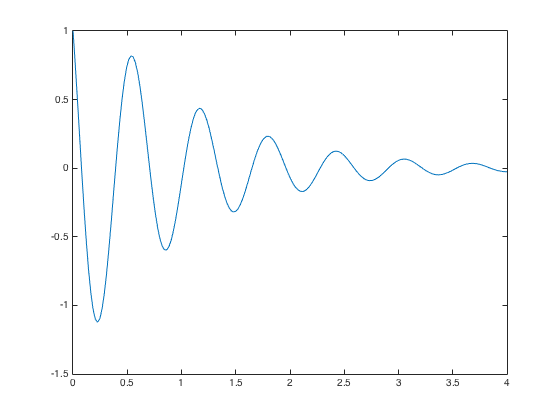
\includegraphics[width = 0.47\textwidth]{zR.png}
\label{fig:subfigure1}}
\quad
\subfigure[Time vs Imaginary Z]{%
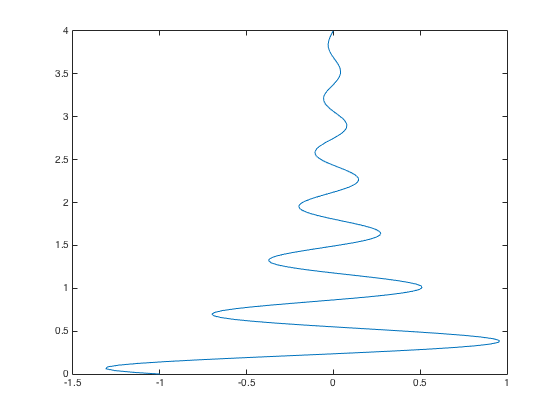
\includegraphics[width=0.47\textwidth]{zi.png}
\label{fig:subfigure2}}
\caption{Z vs Time (and vice versa)}
\label{fig:figure}
\end{figure}

\question Square Spiral
\begin{solution}
Working in the complex plane, we can write the function as a series:
\[
1 + 1i - 1\left(\frac{1}{2}\right) - 1\left(\frac{1}{2}\right)\left(\frac{1}{3}\right)i + 1\left(\frac{1}{2}\right)\left(\frac{1}{3}\right)\left(\frac{1}{4}\right) + ...
\]
which can be separated into a real sum and an imaginary sum:
\begin{align*}
&\left(1 - 1\left(\frac{1}{2}\right) + 1\left(\frac{1}{2}\right)\left(\frac{1}{3}\right)\left(\frac{1}{4}\right) - \cdots \right) + i\left(1 - 1\left(\frac{1}{2}\right)\left(\frac{1}{3}\right) + 1\left(\frac{1}{2}\right)\left(\frac{1}{3}\right)\left(\frac{1}{4}\right)\left(\frac{1}{5}\right) - \cdots \right) \\
&= \sum_{n=0}^{\infty} \frac{1}{(2n)!}(-1)^n + i\sum_{n=0}^{\infty} \frac{1}{(2n+1)!}(-1)^n
\end{align*}
These sums are familiar ones - almost.  The real one is just $\cos{1}$.  The second one has opposite signs of what one is used to and an extra $1$, but subtracting one and multiplying the difference by -1 gives $\sin{1}$, so the imaginary sum is $1 - \sin{1}$.  Thus, the curve will converge to the point $\cos{1} + (1 - \sin{1})i$

\end{solution}

\end{questions}
\end{document}